
% \begin{frame}{Dynamics } 

    % Before Newton, there was Kepler ... 

    % And before dynamics, there was kinematics. 

%     We can predict the final position of a satellite given its initial state and time of flight (TOF). 
    
%     \begin{figure}
%         \centering
%         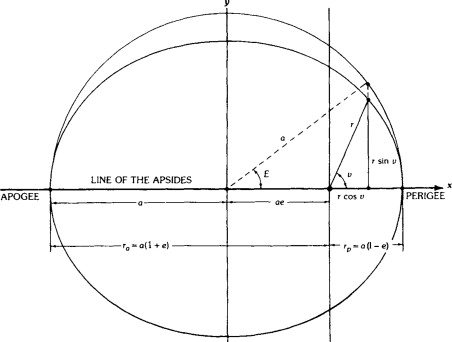
\includegraphics[width=0.6\textwidth]{pres_images/kepler_ellipse.jpg}
%         \caption{Kepler's 2nd Law}
%         \label{fig:kepler_ellipse}
%     \end{figure}
    
% \end{frame}

\begin{frame}{Dynamics }

    In 1601, Johannes Kepler inherited the data of the recently deceased astronomer Tycho Brahe. 
    % 
    By studying Brahe's methodical and precise observations of the night sky, Kepler was able to devise his \textbf{3 laws of planetary motion}:  
    % 
    \begin{enumerate}
        \item Planets move in elliptical orbits with the Sun as a focus 
        \item A planet covers the same area of space in the same amount of time no matter where it is in its orbit 
        \item A planet's orbital period is proportional to the size of its orbit (its semi-major axis)
    \end{enumerate}
    
\end{frame} 

\begin{frame}{Dynamics }

    Using Kepler's laws, we can predict the final position of a celestial body given its initial state and time of flight (TOF). 

    To illustrate, we first describe how to parameterize an orbit using elliptical geometry. 

    \begin{figure}
        \centering
        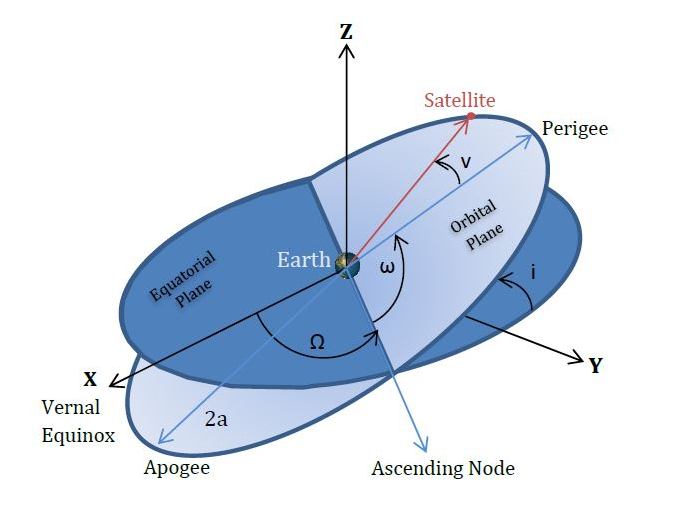
\includegraphics[width = 0.6\textwidth]{pres_images/orbital_elements.png}
        \caption{Keplerian Elements}
        \label{fig:orbital_elements}
    \end{figure}
    
\end{frame} 

\begin{frame}{Dynamics } 

    Additional parameters must be introduced to relate the position of an orbiting body with the time of flight. 

    \begin{figure}
        \centering
        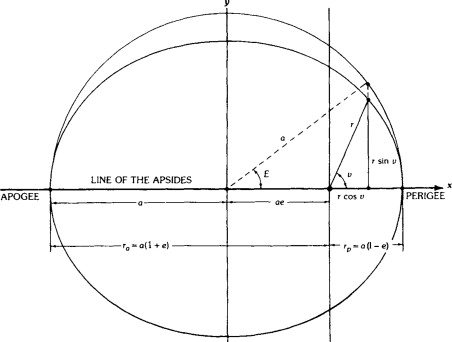
\includegraphics[width=0.6\textwidth]{pres_images/kepler_ellipse.jpg}
        \caption{Keplerian Orbit}
        \label{fig:kepler_orbit}
    \end{figure}

\end{frame} 

\begin{frame}{Dynamics}
        
    For elliptical orbits, we define the eccentric anomaly $E$ as 
% 
    \begin{equation}
        tan \frac{E}{2} = \sqrt{ \frac{1-e}{1+e} } tan \frac{\nu}{2}, 
        \label{eq:E_nu}
    \end{equation}
% 
    and the position of the orbiting body relates to its semimajor axis $a$ and eccentric anomaly via 
% 
    \begin{equation}
        r = a( 1 - e cos E ). 
    \end{equation} 

    To propagate an orbit using Kepler's equation given TOF, $\mathbf{r}_0$, and $\mathbf{v}_0$, first convert the state to Keplerian elements $a$, $e$, $i$, $\omega$, $\Omega$, and $\nu_0$. 

\end{frame}

\begin{frame}{Dynamics }
    
    We define the mean motion, or the average angular speed required for a body to complete one orbit, as  
% 
    \begin{equation}
        n = \sqrt{ \frac{\mu}{|a|^3} }, 
    \end{equation}
% 
    and determine the initial eccentric anomaly $E_0$ from the initial true anomaly $\nu_0$ via \eqref{eq:E_nu}. 
    The mean anomaly, a convenient uniform measure of how far around its orbit a body has progressed since perapsis, can then be propagated 
% 
    \begin{align}
        M_0 & = E_0 - e * sin(E_0) \\ 
        M_f & = M_0 + n * TOF . 
    \end{align}
    
\end{frame} 

\begin{frame}{Dynamics } 

    Eccentric anomaly is related to mean anomaly through \textbf{Kepler's equation} 
% 
    \begin{equation}
        M = E - sin E, 
        \label{eq:kepler_eq}
    \end{equation}
% 
    which can be conveniently solved in one direction but requires an iterative procedure in the other direction (Newton-Raphson commonly used). 
    
    We use Kepler's equation to find $E_f$, the final eccentric anomaly, and finally compute the final position $\nu_f$ through the relation described in \eqref{eq:E_nu}. 
% 
    % \begin{equation}
    %     \nu = 2 tan^{-1} \Bigg( \sqrt{ \frac{1+e}{1-e} } tan \Big( \frac{E}{2} \Big) \Bigg)   
    % \end{equation}
% 
    In general, the time of flight equation using Kepler's laws is  
% 
    \begin{equation}
        t - t_0 = \sqrt{ \frac{a^3}{\mu} } ( E - E_0 - e sin( E - E_0 ) ) . 
    \end{equation}
    
\end{frame} 

\begin{frame}{Dynamics}

    Important note: this formulation suffers from singularities. 

    A standard way to remove singularities is to perform a change of variable reformulation known as the \textbf{Sundman transformation} which results in a time-of-flight equation valid for all conic orbits 

    \begin{equation}
        r = \sqrt{\mu} \frac{dt}{dx} = x^2 C + \frac{ \mathbf{r}_0 \cdot \mathbf{v}_0 }{ \sqrt{\mu} } x (1 - z S) + r_0 (1 - z C) , 
    \end{equation} 

    where $x$ is known as the universal variable and $ z = x^2 / a $. $C$ and $S$ are called Stumpff functions which are used for analyzing orbits using the universal variable formulation.  

    % \begin{equation}
    %     C = \frac{1 - \sqrt{z}}{z} = 
    % \end{equation}

    The universal variable formulation was very time-consuming and not used in this work, but it is the better method. 
    
\end{frame} 


\begin{frame}{Dynamics }

    % An orbit can be completely characterized by its position and velocity.  
    % Given an initial and target position, let's say we wish to determine an initial velocity vector and time of flight to parameterize the trajectory. 

    Finding the minimum energy orbit, or the ellipse that achieves the smallest possible semimajor axis, is called Lambert's Problem. 

    \begin{figure}
        \centering
        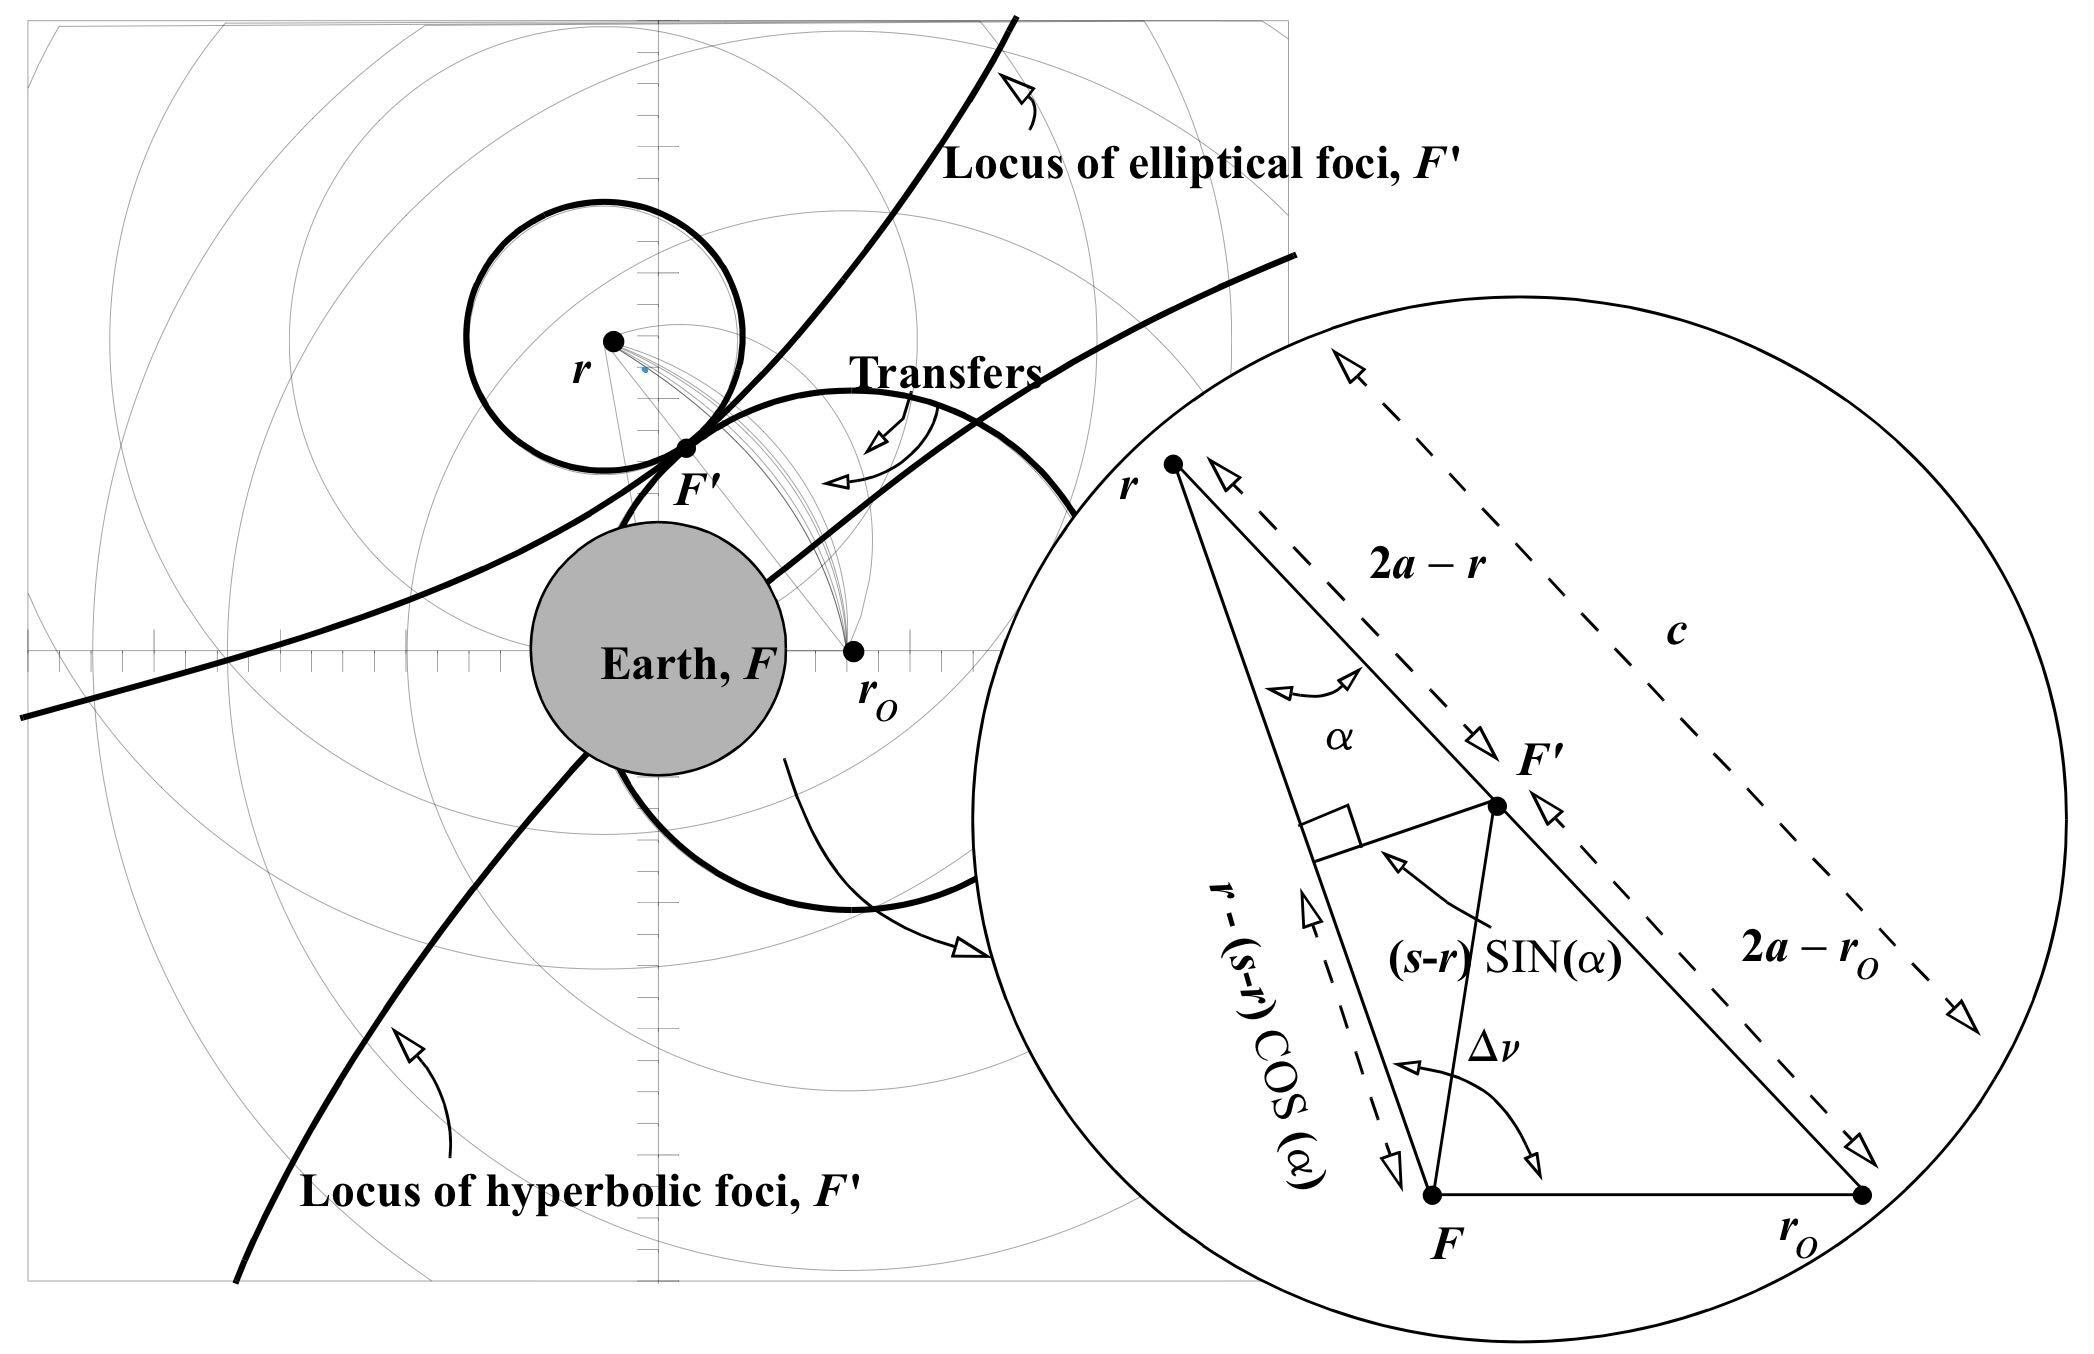
\includegraphics[width = 0.65\textwidth]{pres_images/lambert.jpg}
        \caption{Geometry for the Lambert Problem}
        \label{fig:lambert}
    \end{figure}
    
\end{frame} 

\begin{frame}{Dynamics }

    Using the parameters defined in Figure \ref{fig:lambert}, we can solve for the initial velocity $ \bar{v}_0 $ and time of flight $ t_{min} $. 
    
    \begin{algorithm}[H]
    \begin{algorithmic}[1]
        \STATE $ cos(\Delta \nu) = \frac{ \bar{r}_0 \cdot \bar{r} }{ r_0 r } $ 
        \STATE $ c = \sqrt{ r_0^2 + r^2 - 2 r_0 r cos(\Delta \nu) } $
        \STATE $ s = \frac{ r_0 + r + c }{ 2 } $
        \STATE $ a_{min} = \frac{s}{2} $, $ p_{min} = \frac{ r_0 r }{ c } ( 1 - cos(\Delta \nu) ) $, $ e_{min} = \sqrt{ 1 - \frac{ 2 p_{min} }{ s } } $ 
        \STATE $ \alpha_{min} = \pi $, $ sin( \frac{ \beta_{min} }{ 2 } ) = \sqrt{ \frac{ s - c }{ s } } $ 
        \STATE $ t_{min (amin) } = \sqrt{ \frac{ a^3_{min} }{ \mu } } [ \alpha_{min} \pm ( \beta_{min} - sin( \beta_{min} ) ] $ 
        \STATE $ t_{ min (absolute) } = \frac{1}{3} \sqrt{\frac{2}{\mu}} [ s^{3/2} - ( s - c )^{3/2} ] $ 
        \STATE $ \bar{v}_0 = \frac{ \sqrt{\mu p_{min}} }{ r_0 r sin( \Delta \nu ) } [ \bar{r} - ( 1 - \frac{r}{p_{min}} \{ 1 - cos( \Delta \nu ) \} ) \bar{r}_0 ] $
        \end{algorithmic}
    \caption{Lambert's Problem---Minimum Energy}
    \label{alg:seq}
    \end{algorithm}
    
\end{frame}

